\section{Frontend Architecture and Implementation}

The presentation layer of the DBaaS platform is engineered to abstract the inherent complexities of multi-tenant database management behind an intuitive, declarative user interface. Rather than exposing users to raw Kubernetes manifests or complex SQL DDL commands, the frontend translates user interactions into deterministic API payloads. The architecture strictly adheres to a unidirectional data flow, ensuring that the UI remains a reactive reflection of the backend's state machine.
\subsection{Frontend Development Stack}
The frontend implementation has been evolved to support advanced database operations. The core stack includes:
\begin{itemize}
    \item \textbf{Framework:} Flutter Web (CanvasKit).
    \item \textbf{State Management:} BLoC/Cubit for complex reactive flows.
    \item \textbf{Visualization:} Mermaid.js for ERDs and fl\_chart for telemetry.
    \item \textbf{Networking:} HTTP package with custom interceptors for session management.
\end{itemize}
\subsection{Architectural Rationale: Flutter for the Web}

To construct a highly responsive, single-codebase application capable of rendering complex data grids and interactive schema diagrams, the presentation layer was implemented using \textbf{Flutter}. While traditional Document Object Model (DOM) based frameworks (e.g., ReactJS, VueJS) are prevalent, Flutter's CanvasKit rendering engine was selected for its ability to bypass DOM manipulation bottlenecks, achieving consistent pixel-perfect rendering across all environments.

Table~\ref{tab:flutter_comparison} summarizes the architectural justifications for selecting Flutter over conventional DOM-based web technologies for this specific DBaaS use case.

\begin{table}[ht]
\centering
\caption{Comparison of Flutter Web with Other Web Technologies}
\label{tab:flutter_comparison}
\renewcommand{\arraystretch}{1.3}
\begin{tabular}{|l|c|c|c|c|}
\hline
\textbf{Aspect} & \textbf{Flutter Web} & \textbf{ReactJS} & \textbf{Angular} & \textbf{VueJS} \\
\hline
Single Codebase & \ding{51} & \ding{55} & \ding{55} & \ding{55} \\
\hline
Pixel-perfect UI & \ding{51} & \ding{55} & \ding{55} & \ding{55} \\
\hline
Hot Reload / Fast Development & \ding{51} & \ding{51} & \ding{55} & \ding{51} \\
\hline
Enterprise Ready & \ding{55} & \ding{51} & \ding{51} & \ding{55} \\
\hline
Lightweight & \ding{55} & \ding{55} & \ding{55} & \ding{51} \\
\hline
Large Community Support & \ding{51} & \ding{51} & \ding{51} & \ding{51} \\
\hline
Best for Animations & \ding{51} & \ding{55} & \ding{55} & \ding{55} \\
\hline
Easy to Learn & \ding{55} & \ding{55} & \ding{55} & \ding{51} \\
\hline
\end{tabular}
\end{table}
\newpage
\section{Platform Features and UI Coverage}

This section highlights the functional modules exposed through the Flutter frontend and notes areas where UI coverage is still partial relative to the backend API.

\subsection{Implemented Features}

% --- 1. Authentication ---
\subsubsection*{Authentication and User Identity Management}
The authentication module provides secure user access through simple login and registration interfaces.

Main features include:
\begin{itemize}
    \item Switching between \textit{Sign In} and \textit{Sign Up} within the same interface.
    \item Basic validation of email and password inputs.
    \item Secure communication with the backend for authentication and session handling.
    \item Support for password recovery and account restoration.
\end{itemize}


\begin{figure}[H]
    \centering
    \begin{subfigure}[b]{0.48\textwidth}
        \centering
        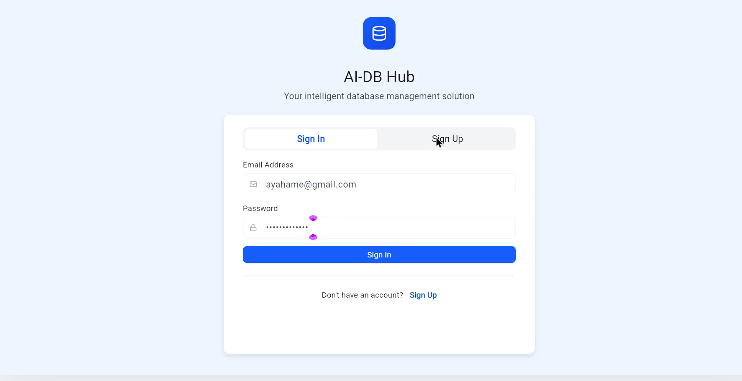
\includegraphics[width=\textwidth]{images/UI/login.png}
        \caption{Login Interface}
    \end{subfigure}
    \hfill
    \begin{subfigure}[b]{0.48\textwidth}
        \centering
        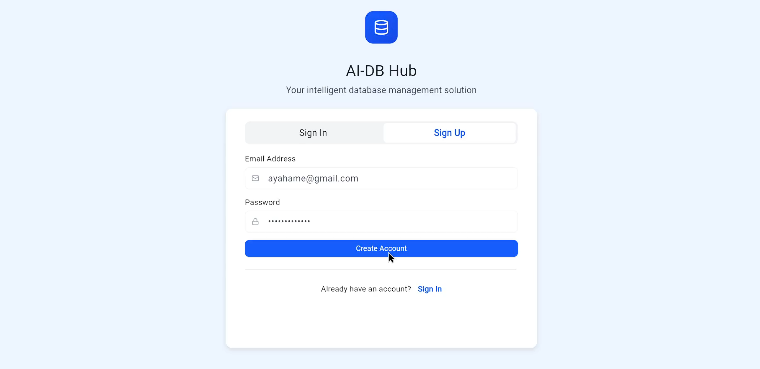
\includegraphics[width=\textwidth]{images/UI/signup.png}
        \caption{Registration Interface}
    \end{subfigure}
    \caption{Authentication module features and user onboarding workflow.}
\end{figure}

% --- 2. Home Tab & Project Creation ---
\subsubsection*{Project Provisioning and Lifecycle Management}
The platform simplifies database project creation and management through an easy and user-friendly workflow.

Key features include:
\begin{itemize}
    \item Creating projects by specifying the project name, database type, and DB password.
    \item Displaying active projects in a dynamic dashboard with quick access to project operations.
    \item Providing administrative actions such as deleting, exporting, and restoring projects.
\end{itemize}

\begin{figure}[H]
    \centering
    \begin{subfigure}[b]{0.32\textwidth}
        \centering
        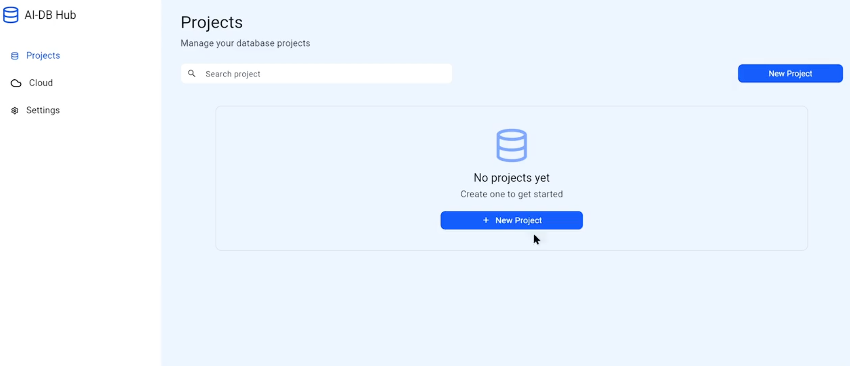
\includegraphics[width=\textwidth]{images/UI/empty_homescreen.png}
        \caption{Initial Empty State}
    \end{subfigure}
    \hfill
    \begin{subfigure}[b]{0.32\textwidth}
        \centering
        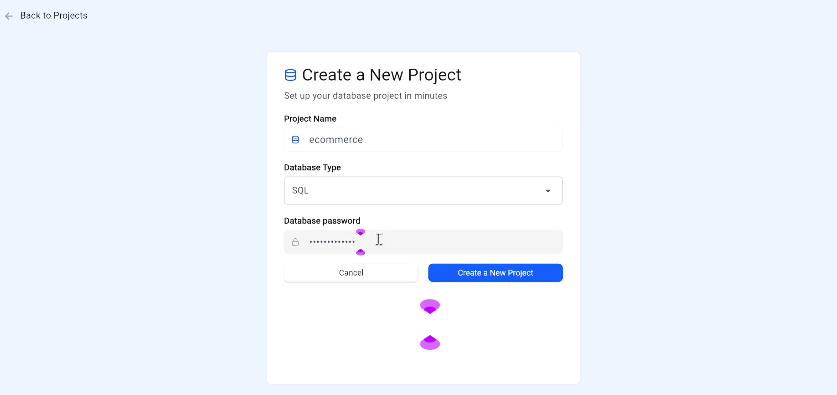
\includegraphics[width=\textwidth]{images/UI/create sql project.png}
        \caption{Create SQL Project }
    \end{subfigure}
    \hfill
    \begin{subfigure}[b]{0.32\textwidth}
        \centering
        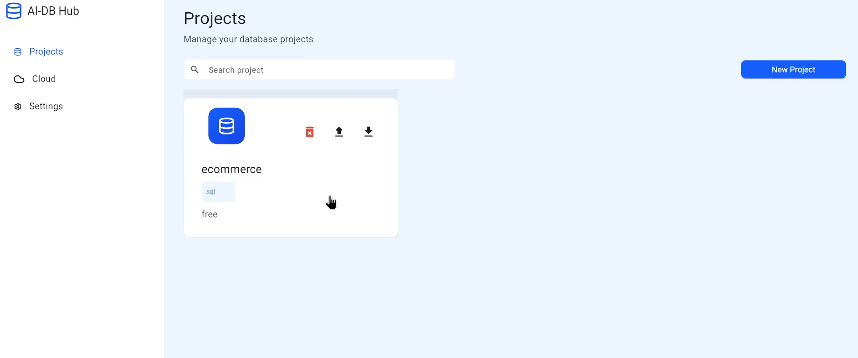
\includegraphics[width=\textwidth]{images/UI/display project in home.png}
        \caption{Project Overview Card}
    \end{subfigure}
    \caption{Workflow for database project creation and administrative overview.}
\end{figure}
\subsubsection*{Relational Schema Design \& Table Management}
The SQL workbench provides an easy interface for creating and managing relational database schemas without writing SQL code.

Key features include:
\begin{itemize}
    \item Creating tables with columns, constraints, and relationships through a visual interface.
    \item Displaying all tables and their details in a dashboard for easy navigation and management.
\end{itemize}
\begin{figure}[H]
    \centering
    \begin{subfigure}[b]{0.45\textwidth}
        \centering
        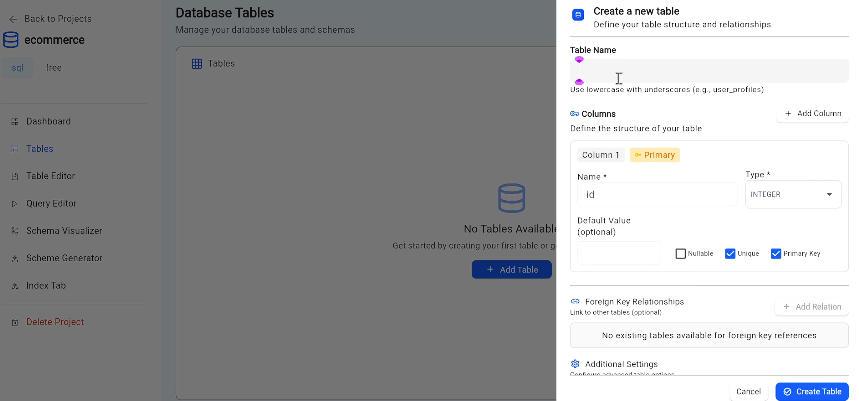
\includegraphics[width=\textwidth]{images/UI/create table.png}
        \caption{Table Creation Modal}
    \end{subfigure}
    \hfill
    \begin{subfigure}[b]{0.45\textwidth}
        \centering
        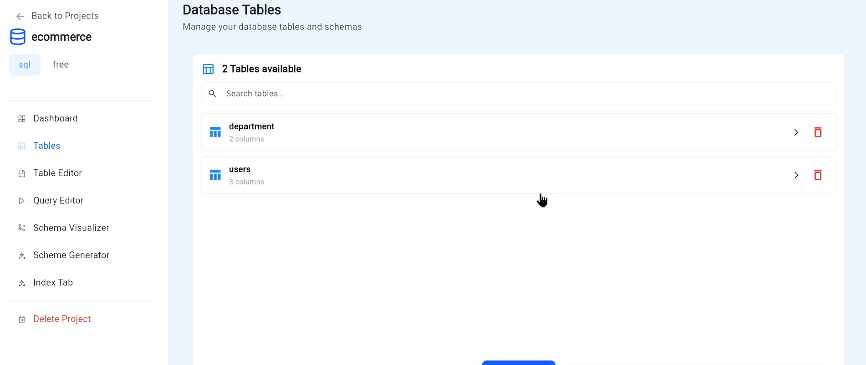
\includegraphics[width=\textwidth]{images/UI/display tables.png}
        \caption{Finalized Schema Overview}
    \end{subfigure}
    \caption{Relational table creation and management workflow.}
\end{figure}
\subsubsection*{Data Manipulation and Content Management}
The \textit{Table Editor} module provides an easy interface for managing database content without writing SQL queries.

The module supports three main functions:

\begin{itemize}
    \item \textbf{Record Manipulation (CRUD):} Users can insert, edit, and delete records through simple forms with basic data validation.
    
    \item \textbf{Schema Updates:} Users can add new columns and modify table structures, with changes reflected immediately in the interface.
    
    \item \textbf{Data Visualization:} The data grid displays table content and automatically updates to reflect the latest changes.
\end{itemize}
\begin{figure}[H]
    \centering
    \begin{subfigure}[b]{0.45\textwidth}
        \centering
        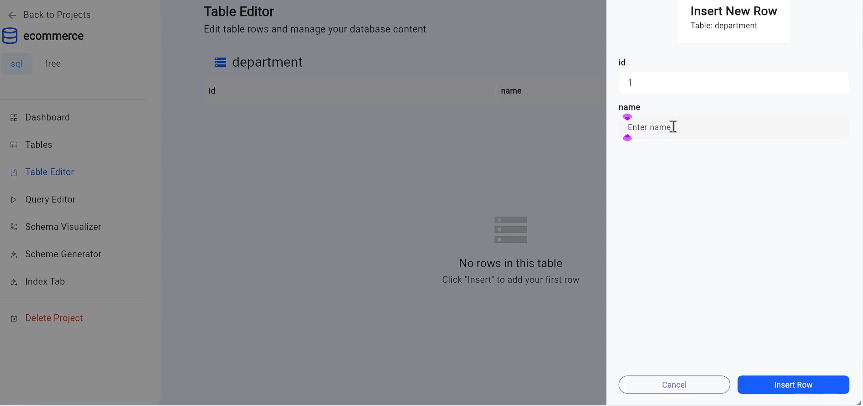
\includegraphics[width=\textwidth]{images/UI/insert row.png}
        \caption{Record Insertion Modal}
    \end{subfigure}
    \hfill
    \begin{subfigure}[b]{0.45\textwidth}
        \centering
        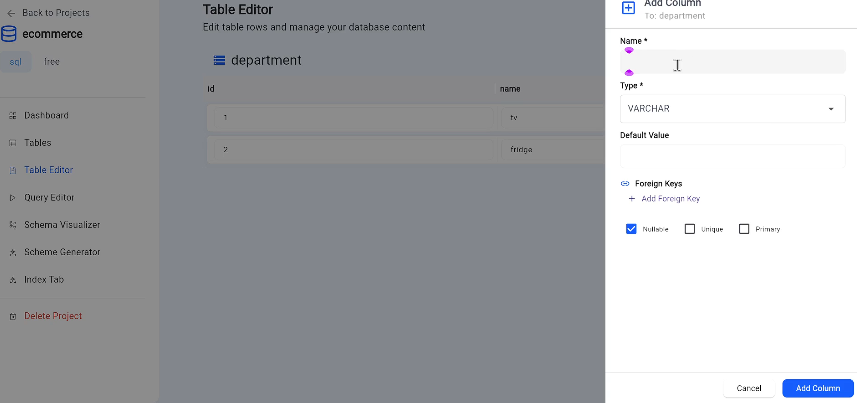
\includegraphics[width=\textwidth]{images/UI/add column.png}
        \caption{Dynamic Column Addition}
    \end{subfigure}
    \vspace{10pt}
    \begin{subfigure}[b]{0.45\textwidth}
        \centering
        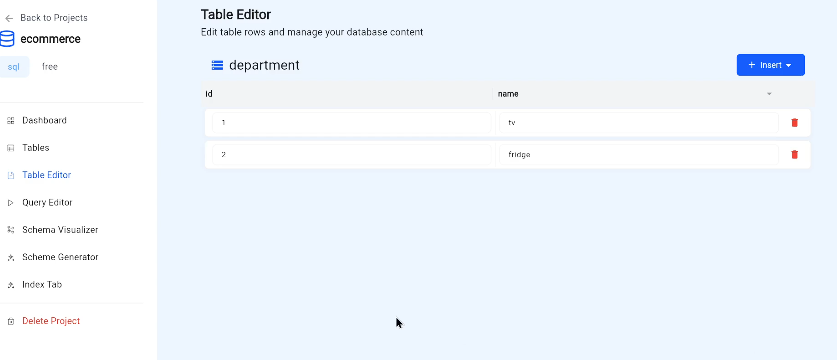
\includegraphics[width=\textwidth]{images/UI/inserted Rows.png}
        \caption{Data Grid Visualization}
    \end{subfigure}
    \caption{The comprehensive workflow for data manipulation and schema management within the platform.}
\end{figure}


\subsubsection*{Interactive Schema Visualization}
The platform includes an \textit{Interactive Schema Visualizer} that provides a graphical representation of database structures and relational dependencies. This feature is powered by the \textit{Mermaid} library, which translates the database schema into dynamic diagrams in real-time.

Key features include:
\begin{itemize}
    \item \textbf{Dynamic Rendering:} Automatically generates and updates entity-relationship diagrams (ERDs) based on real-time database schema changes.
    \item \textbf{Mermaid-powered Visualization:} Leverages the Mermaid syntax to create clean, programmatic, and version-controlled visual documentation of table relationships.

\end{itemize}

\begin{figure}[H]
    \centering
    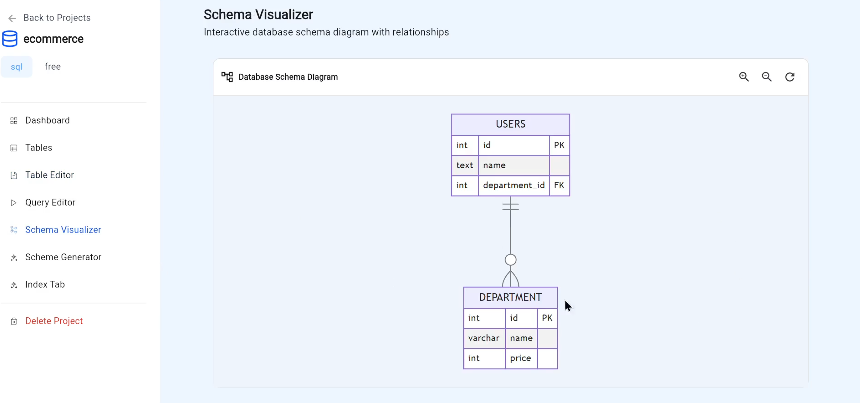
\includegraphics[width=0.9\textwidth]{images/UI/schema_viz.png}
    \caption{Interactive schema visualization rendered via Mermaid, illustrating relational dependencies.}
    \label{fig:schema_viz}
\end{figure}

\subsubsection*{Index Management and Performance Optimization}
The platform provides an \textit{Index Tab} for creating and managing database indexes to improve query performance.

Key features include:
\begin{itemize}
    \item Creating indexes on selected columns through a simple interface.
    \item Displaying and managing all existing indexes within the project.
    \item Supporting database optimization by making index management easier.
\end{itemize}


\begin{figure}[H]
    \centering
    \begin{subfigure}[b]{0.45\textwidth}
        \centering
        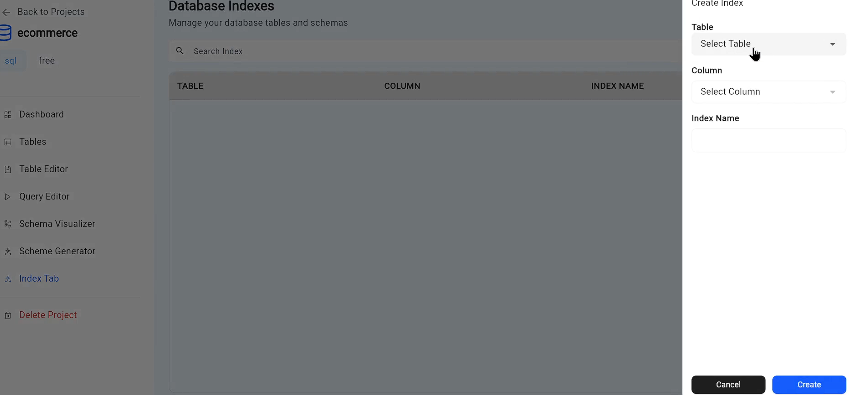
\includegraphics[width=\textwidth]{images/UI/create indexes.png}
        \caption{Index Creation Workflow}
    \end{subfigure}
    \hfill
    \begin{subfigure}[b]{0.45\textwidth}
        \centering
        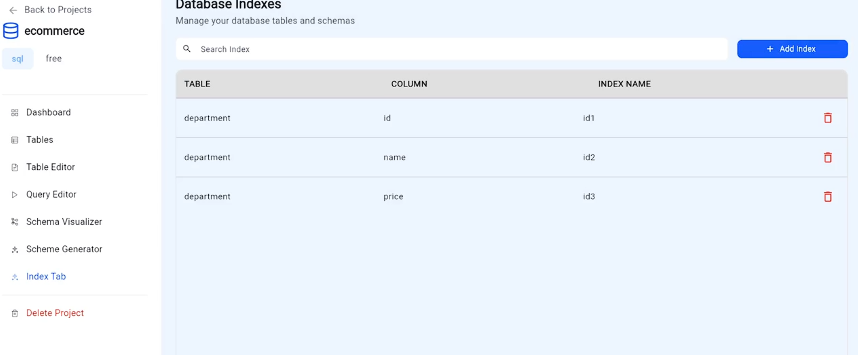
\includegraphics[width=\textwidth]{images/UI/display_indexes.png}
        \caption{Index Inventory Overview}
    \end{subfigure}
    \caption{Index management interface for database performance optimization.}
\end{figure}
\subsubsection*{SQL Query Workbench and Execution Engine}
The platform includes an SQL Query Workbench that allows users to execute custom SQL statements directly on the database.

Key features include:
\begin{itemize}
    \item Writing and executing SQL queries such as \textit{SELECT}, \textit{INSERT}, and \textit{DELETE}.
    \item Automatically displaying query results and reflecting database changes in the interface.
    \item Providing feedback messages about query execution status and errors.
\end{itemize}


\begin{figure}[H]
    \centering
    \begin{subfigure}[b]{0.45\textwidth}
        \centering
        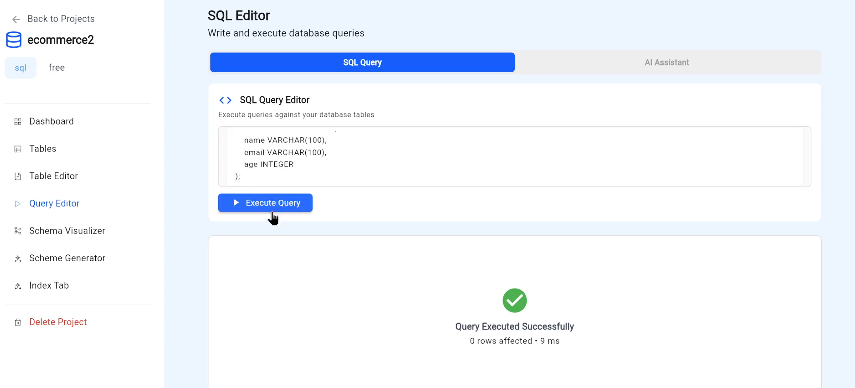
\includegraphics[width=\textwidth]{images/UI/create table query.png}
        \caption{Query Execution Interface}
    \end{subfigure}
    \hfill
    \begin{subfigure}[b]{0.45\textwidth}
        \centering
        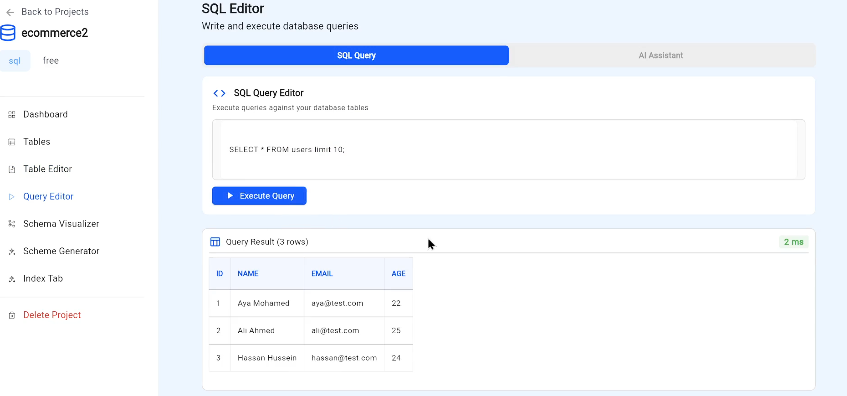
\includegraphics[width=\textwidth]{images/UI/select query.png}
        \caption{Result Grid Reflection}
    \end{subfigure}
    \caption{Interactive SQL Query Workbench and result reflection engine.}
\end{figure}



\subsubsection*{Real-time Telemetry and System Monitoring}
The platform includes a monitoring dashboard that provides real-time insights into database performance and resource usage.

Key features include:
\begin{itemize}
    \item Displaying live metrics such as CPU, memory, and I/O usage.
    \item Providing an overview of the database health and performance.
    \item Offering interactive charts for analyzing resource consumption over time.
\end{itemize}
\begin{figure}[H]
    \centering
    \begin{subfigure}[b]{0.48\textwidth}
        \centering
        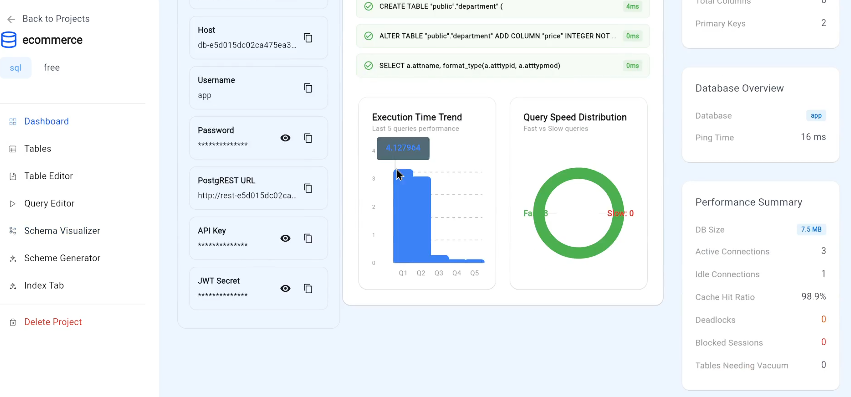
\includegraphics[width=\textwidth]{images/UI/dash_charts.png}
        \caption{Resource consumption metrics (CPU/RAM).}
    \end{subfigure}
    \hfill
    \begin{subfigure}[b]{0.48\textwidth}
        \centering
        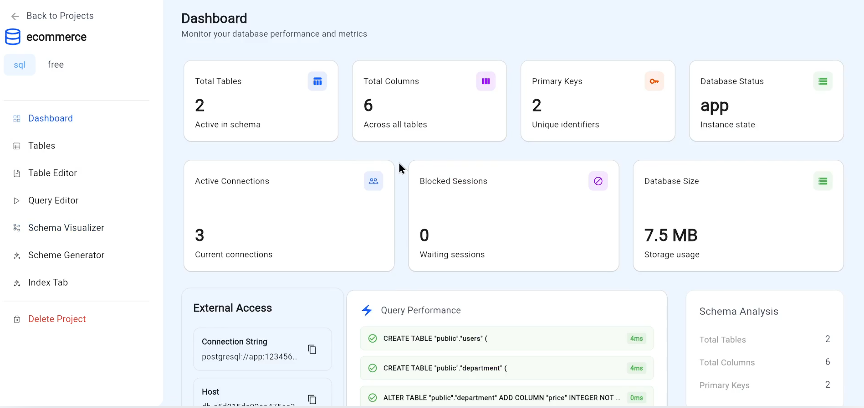
\includegraphics[width=\textwidth]{images/UI/full_dash.png}
        \caption{Integrated telemetry dashboard.}
    \end{subfigure}
    \caption{Real-time system monitoring and performance analytics dashboard.}
\end{figure}
\subsubsection*{Automated Schema Generation and State Reflection}
The platform includes an automated schema generation module that helps users create database structures and review changes before applying them.

Key features include:
\begin{itemize}
    \item Generating database schemas based on user requirements.
    \item Automatically updating the interface to reflect database changes in real time.
    \item Validating structural changes before applying them to prevent conflicts.
\end{itemize}


\begin{figure}[H]
    \centering
    \begin{subfigure}[b]{0.45\textwidth}
        \centering
        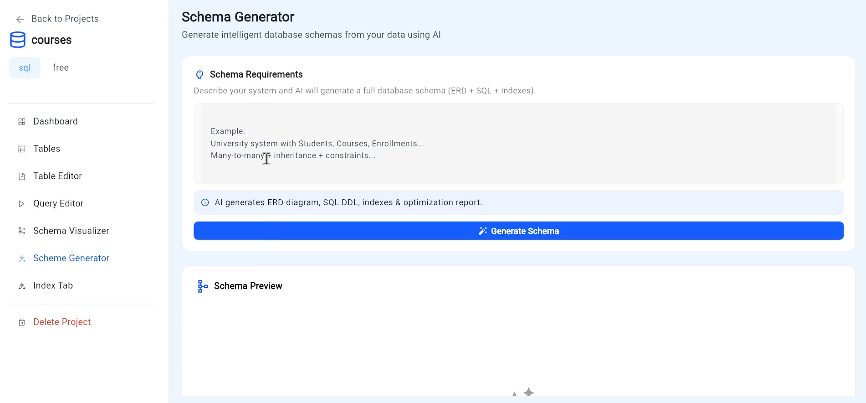
\includegraphics[width=\textwidth]{images/UI/schema_generation.png}
        \caption{Automated Schema Generation Tool}
    \end{subfigure}
    \hfill
    \begin{subfigure}[b]{0.45\textwidth}
        \centering
        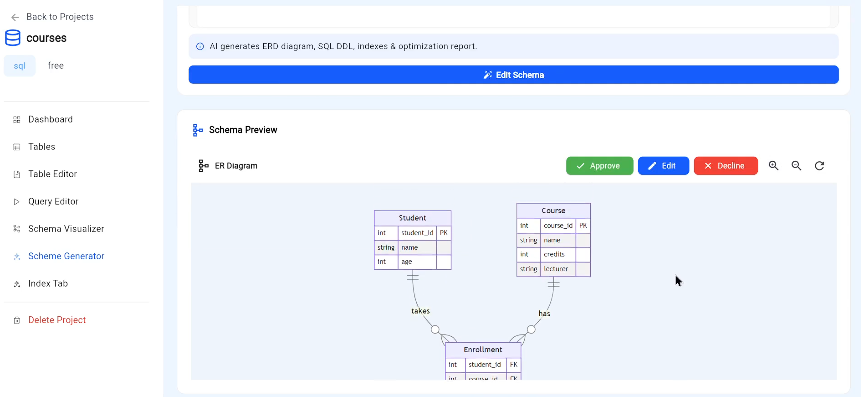
\includegraphics[width=\textwidth]{images/UI/preiview & approve.png}
        \caption{Preview \& Approval Workflow}
    \end{subfigure}
    \vspace{10pt}
    \begin{subfigure}[b]{0.45\textwidth}
        \centering
        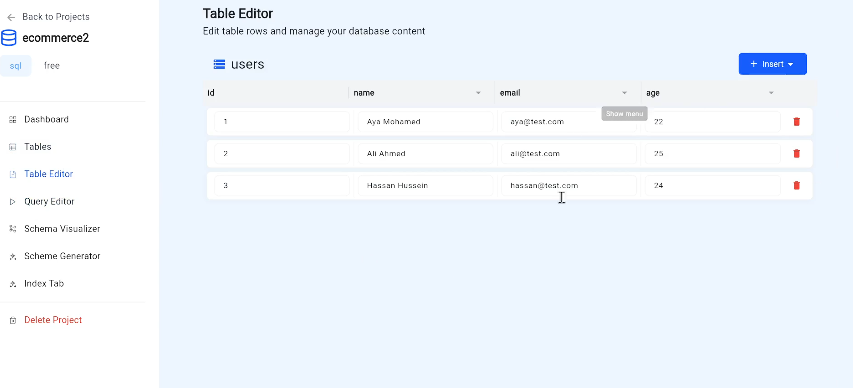
\includegraphics[width=\textwidth]{images/UI/reflect on table.png}
        \caption{Synchronized Table Navigation}
    \end{subfigure}
    \caption{Workflow for automated schema synthesis and real-time state reflection.}
\end{figure}
\subsubsection*{Data Portability and Backup Strategy}
The platform includes backup and export tools that help users manage and protect their data.

Key features include:
\begin{itemize}
    \item Exporting database content as SQL or CSV files.
    \item Providing a secure workflow for project deletion with confirmation steps.
    \item Supporting backup and recovery by enabling easy data export and storage.
\end{itemize}
\begin{figure}[H]
    \centering
    \begin{subfigure}[b]{0.45\textwidth}
        \centering
        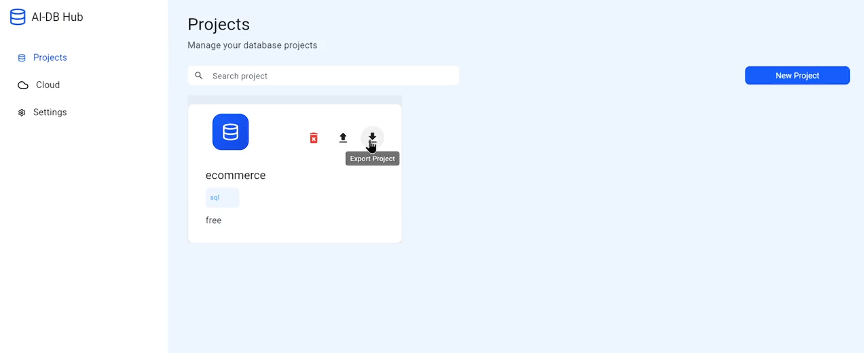
\includegraphics[width=\textwidth]{images/UI/export.png}
        \caption{Data Export and Backup Module}
    \end{subfigure}
    \hfill
    \begin{subfigure}[b]{0.45\textwidth}
        \centering
        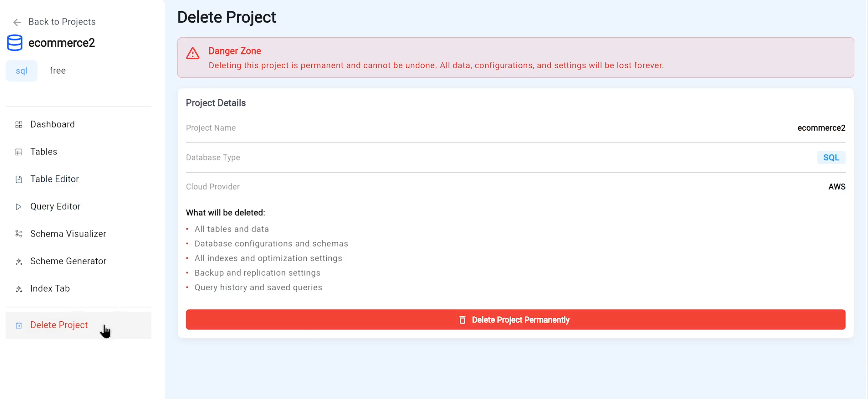
\includegraphics[width=\textwidth]{images/UI/delete project.png}
        \caption{Secure Project Termination Modal}
    \end{subfigure}
    \caption{Data portability and lifecycle management workflow.}
\end{figure}
\subsection*{NoSQL Project Provisioning Workflow}
The platform provides a simple workflow for creating and initializing NoSQL database projects.

Key features include:
\begin{itemize}
    \item Creating projects by specifying the project name and NoSQL database type.
    \item Using a unified workflow for both SQL and NoSQL project provisioning.
    \item Automatically preparing the workspace after project creation.
\end{itemize}


\begin{figure}[H]
    \centering
    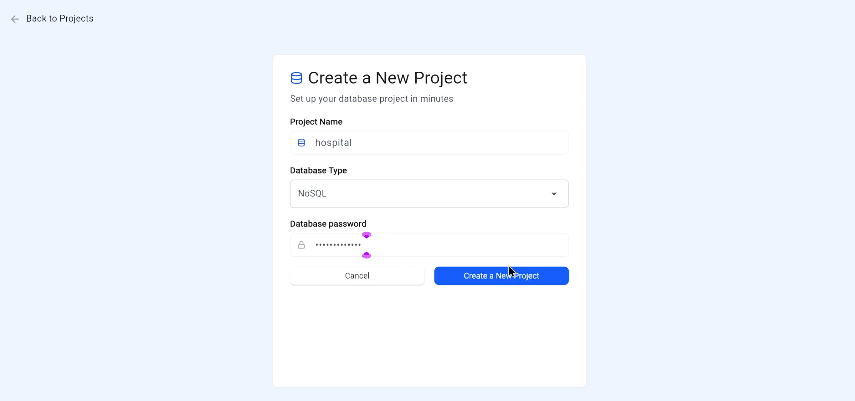
\includegraphics[width=0.7\textwidth]{images/UI/create no sql project.png}
    \caption{Interface for initiating NoSQL database projects.}
\end{figure}
\subsubsection*{NoSQL Collection Management and Document Operations}
To support the agile nature of document-oriented databases, the platform includes a specialized interface for managing collections and individual JSON documents. This module enables developers to define, query, and manipulate data structures without the rigidity of traditional relational tables.

Key functional capabilities include:
\begin{itemize}
    \item \textbf{Dynamic Collection Creation:} Users can instantiate new collections through an intuitive interface that streamlines the definition of storage boundaries, providing an immediate environment for document ingestion.
    \item \textbf{Collection Overview Dashboard:} A comprehensive management view that lists all active collections, displaying document counts and metadata. This dashboard acts as the central hub for monitoring data growth and structural organization within the NoSQL project.
\end{itemize}

\begin{figure}[H]
    \centering
    \begin{subfigure}[b]{0.45\textwidth}
        \centering
        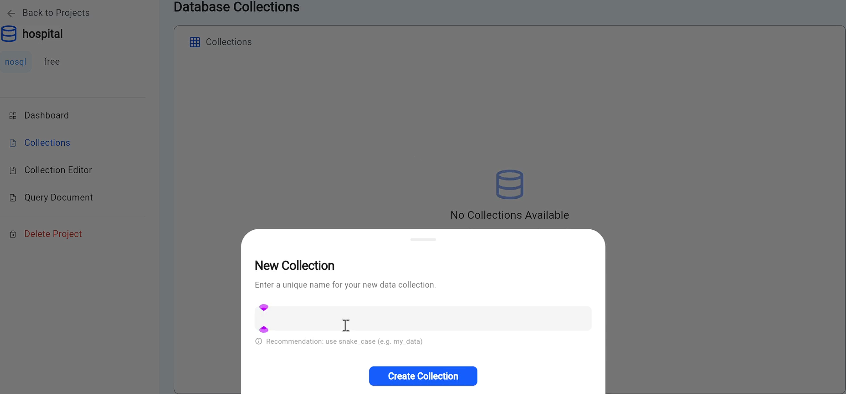
\includegraphics[width=\textwidth]{images/UI/create collection.png}
        \caption{Collection Creation Interface}
    \end{subfigure}
    \hfill
    \begin{subfigure}[b]{0.45\textwidth}
        \centering
        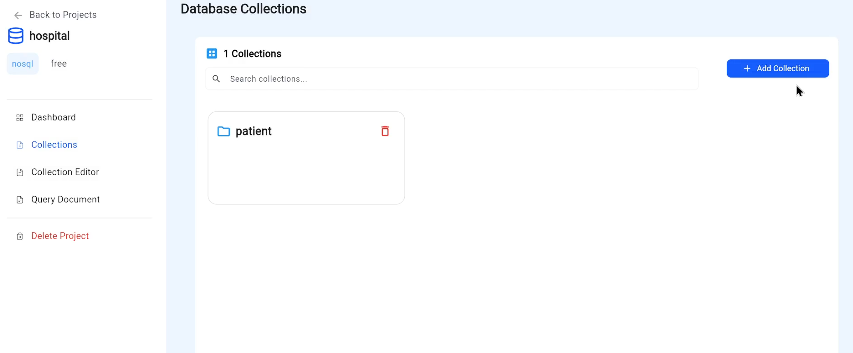
\includegraphics[width=\textwidth]{images/UI/display collections.png}
        \caption{Collection Inventory Dashboard}
    \end{subfigure}
    \caption{Workflow for managing NoSQL document collections and storage structures.}
\end{figure}
\subsubsection*{Document Manipulation and Edit Workflow}
The platform provides a dedicated interface for document-level CRUD operations in NoSQL projects. This module abstracts the complexities of JSON formatting, allowing users to modify data structures within collections with high precision.

Key features include:
\begin{itemize}
    \item \textbf{Intuitive Document Creation:} A streamlined interface allows users to add new JSON documents to a collection. The system provides real-time syntax highlighting and structure validation to prevent malformed data insertion.
    \item \textbf{Reactive Document Editor:} The edit workflow features a modal-based document viewer that parses existing JSON data. Users can perform granular updates on specific fields, and upon submission, the backend reflects these changes across the entire collection state.
    \item \textbf{Validation-Aware Interaction:} Every insertion or update is subjected to a schema-validation layer, ensuring that incoming documents adhere to expected field types and constraints defined within the collection context.
\end{itemize}

\begin{figure}[H]
    \centering
    \begin{subfigure}[b]{0.45\textwidth}
        \centering
        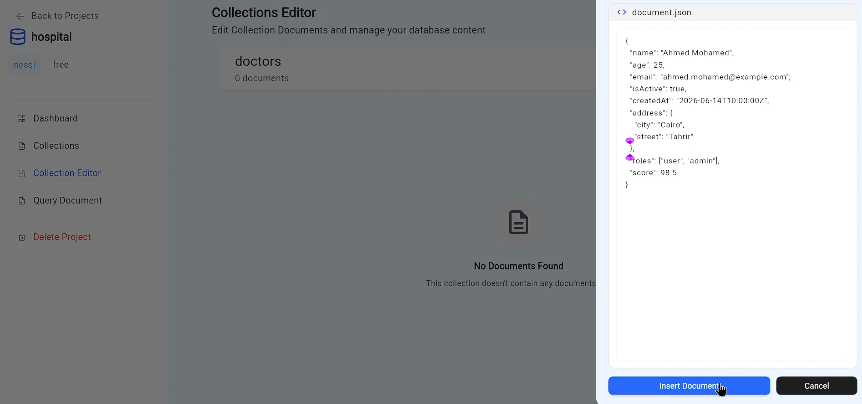
\includegraphics[width=\textwidth]{images/UI/add doc.png}
        \caption{Document Insertion Modal}
    \end{subfigure}
    \hfill
    \begin{subfigure}[b]{0.45\textwidth}
        \centering
        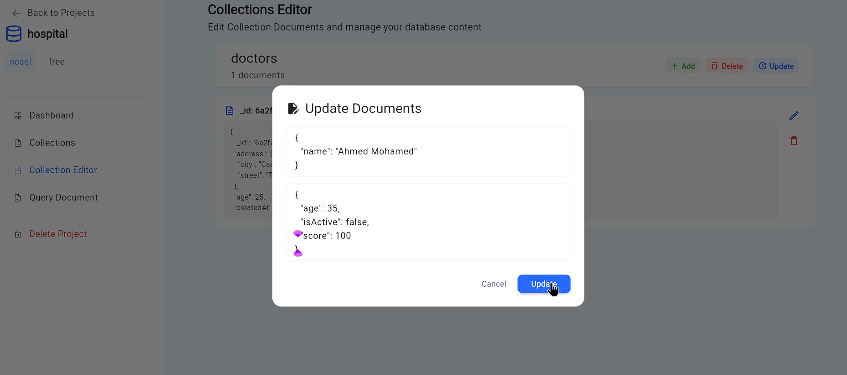
\includegraphics[width=\textwidth]{images/UI/update docs.png}
        \caption{Document Update Workflow}
    \end{subfigure}
    \caption{Workflow for managing NoSQL document content within collections.}
\end{figure}
\subsubsection*{Dynamic Field Management in NoSQL Documents}
The platform's NoSQL editor supports an agile approach to data modeling through dynamic field management. This allows developers to modify the structure of JSON documents in real-time, catering to evolving application requirements without structural downtime.

Key features include:
\begin{itemize}
    \item \textbf{Dynamic Attribute Injection:} Users can add, rename, or delete fields within a document seamlessly. The interface provides a user-friendly modal that handles type identification (String, Integer, Boolean, Nested Objects), ensuring valid JSON syntax during input.
    \item \textbf{Schema-less Extension:} Unlike traditional databases that require an \textit{ALTER TABLE} statement, this feature allows for "on-the-fly" schema extension. This is particularly beneficial for rapid prototyping, where document structures may need to expand as new features are developed.
    \item \textbf{Data Integrity Safeguards:} Even within a schema-less environment, the platform performs client-side validation to ensure that newly added fields do not conflict with existing document integrity or naming conventions.
\end{itemize}

\begin{figure}[H]
    \centering
    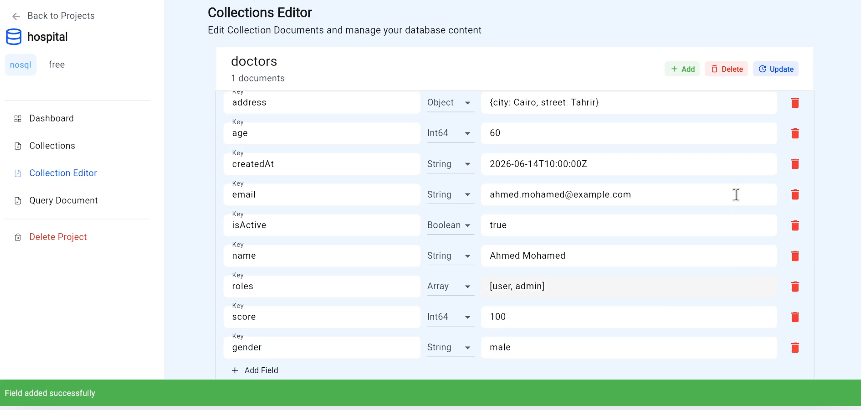
\includegraphics[width=0.6\textwidth]{images/UI/add feild.png}
    \caption{Dynamic field addition interface for NoSQL documents.}
\end{figure}
\subsubsection*{NoSQL Query Workbench}
To provide developers with advanced data retrieval capabilities, the platform includes a dedicated \textit{Query Workbench} for NoSQL collections. This module bridges the gap between abstract document management and powerful data querying.

Key features include:
\begin{itemize}
    \item \textbf{Syntax-Optimized Query Editor:} The interface supports standard NoSQL query syntax (e.g., MongoDB-style filters), allowing users to define precise criteria for data retrieval.
    \item \textbf{Instant Result Reflection:} Upon execution, the workbench utilizes a reactive engine to parse the returned JSON result sets. The UI dynamically generates a structured grid, ensuring that query outputs are displayed clearly and remain navigable for further analysis.
    \item \textbf{Operational Feedback Loop:} Each query operation is accompanied by real-time status indicators, facilitating rapid debugging and iterative refinement of data retrieval patterns within complex document hierarchies.
\end{itemize}

\begin{figure}[H]
    \centering
    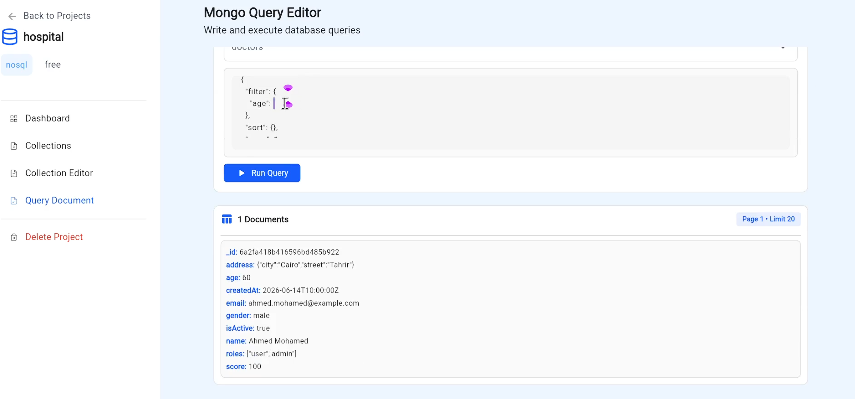
\includegraphics[width=0.7\textwidth]{images/UI/query collection.png}
    \caption{NoSQL Query Workbench interface for precise data retrieval.}
\end{figure}








\subsection{MongoDB Dashboard and Telemetry}
The MongoDB Dashboard provides a comprehensive telemetry suite, ensuring developers have real-time visibility into their NoSQL data stores. The interface is organized into two distinct functional areas:

\begin{itemize}
    \item \textbf{Operational Metrics:} Summary cards offer immediate insights into database growth and activity, tracking document counts, storage utilization, and a 30-day history of CRUD operations (Inserts, Updates, and Deletes). This data is essential for monitoring the lifecycle of the application's data.
    \item \textbf{Connectivity Management:} The dashboard simplifies external integration by explicitly exposing the connection string. This allows users to interface with their managed database instances from external development environments or production applications seamlessly, abstracting the underlying network configuration of the Kubernetes-based storage.
\end{itemize}

\begin{figure}[H]
    \centering
    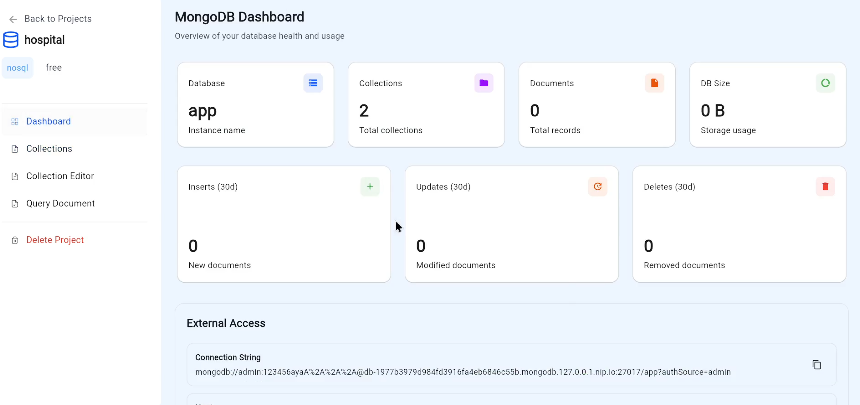
\includegraphics[width=0.9\textwidth]{images/UI/dash_nosql.png}
    \caption{MongoDB Dashboard overview showing operational metrics and external connectivity.}
    \label{fig:nosql_dashboard}
\end{figure}



\section{User Account and System Settings}
The platform provides a comprehensive user settings module, ensuring that account management and personalization are handled securely and intuitively. This module is essential for maintaining user autonomy and platform accessibility.

\subsection{Account Security and Session Management}
The account settings interface centralizes session and identity management, focusing on user-controlled security actions.
\begin{itemize}
    \item \textbf{Secure Authentication Control:} Users have immediate access to administrative actions, including session termination (Log Out) and permanent account removal.
    \item \textbf{Account Deletion Safeguards:} To prevent accidental loss of data and project access, the account deletion workflow is implemented as a protected administrative action, requiring explicit confirmation to ensure the integrity of the user's workspace.
\end{itemize}

\subsection{Personalization and Interface Preferences}
To enhance the usability and accessibility of the platform, we implemented a dedicated appearance and settings panel.
\begin{itemize}
    \item \textbf{Appearance Customization:} The platform supports a flexible UI, allowing users to toggle between different themes (e.g., Light/Dark mode). This is achieved through a reactive theme-provider pattern that updates the UI state globally across the application without requiring a page refresh.
    \item \textbf{System Configuration:} The settings dashboard serves as a unified hub for managing application-wide preferences, ensuring that developers can tailor their workspace to suit their operational needs.
\end{itemize}

\begin{figure}[H]
    \centering
    \begin{subfigure}[b]{0.32\textwidth}
        \centering
        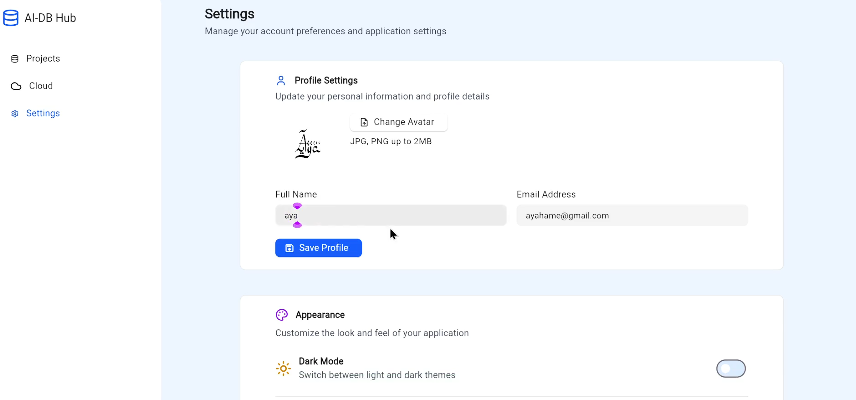
\includegraphics[width=\textwidth]{images/UI/settings.png}
        \caption{Settings Dashboard}
    \end{subfigure}
    \hfill
    \begin{subfigure}[b]{0.32\textwidth}
        \centering
        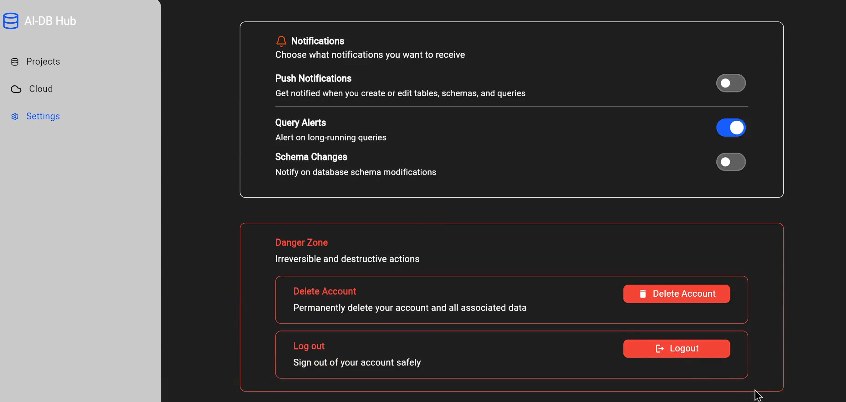
\includegraphics[width=\textwidth]{images/UI/logout and delete acc.png}
        \caption{Account Security Actions}
    \end{subfigure}
    \hfill
    \begin{subfigure}[b]{0.32\textwidth}
        \centering
        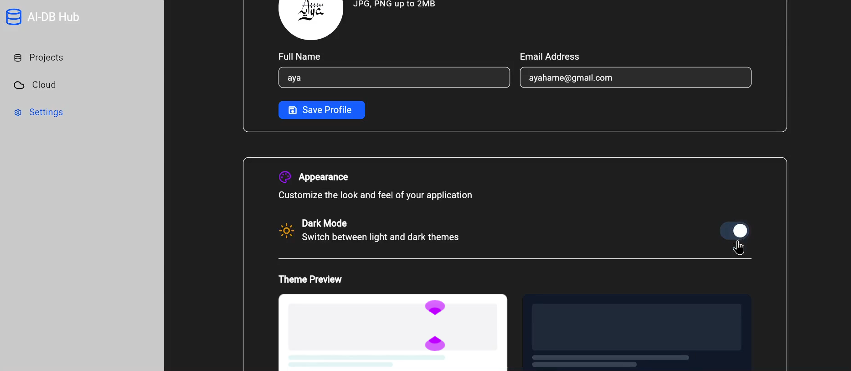
\includegraphics[width=\textwidth]{images/UI/appearance.png}
        \caption{Appearance Preferences}
    \end{subfigure}
    \caption{User account management, security controls, and interface personalization.}
\end{figure}